\documentclass[12pt,aspectratio=169]{beamer}
\usepackage{parskip}
\usepackage{graphicx}
\usepackage{fontspec}
\usepackage{gelasio}
\usecolortheme{dolphin}
\useoutertheme{udec}
\usefonttheme{serif}
\setmainfont{Gelasio}

\definecolor{accent}{RGB}{0,17,88}
\definecolor{background}{RGB}{242,242,242}
\setbeamercolor*{structure}{bg=accent!20,fg=accent}
\setbeamercolor*{normal text}{fg=black,bg=background}


\begin{document}
\begin{beamercolorbox}[wd=\paperwidth,ht=0.55\paperheight,left,leftskip=1em]{palette tertiary}
	\vbox to0.55\paperheight{%
		\vfil
		\Large
		\textbf{Development of a communications}
		\linebreak
		\textbf{protocol between X-Plane and}
		\linebreak
		\textbf{external microcontrollers.}
		\vfil
	}
\end{beamercolorbox}
\begingroup
\setlength{\parskip}{-16pt}
\phantom{a}
\begin{beamercolorbox}[wd=\paperwidth,ht=0.15\paperheight,left,leftskip=1em]{palette primary}
	\vbox to0.15\paperheight{%
		\vfil
		\usebeamerfont{author in title}
		\small
		\textcolor{white}{Germán Quijada}
		\vfil
	}
\end{beamercolorbox}
\hbox{%
	\begin{beamercolorbox}[wd=0.5\paperwidth,ht=0.2255\paperheight,left,leftskip=1em]{white}
		
\includegraphics[height=4.7em]{udec}
	\end{beamercolorbox}
	\begin{beamercolorbox}[wd=0.5\paperwidth,ht=0.2255\paperheight,right,rightskip=5em]{white}
		\scriptsize\today
		\linebreak
		\phantom{aa}
		\linebreak
		\footnotesize
		\phantom{aa}
	\end{beamercolorbox}
}
\endgroup
%
\begin{frame}{X-Plane}
	\begin{columns}
	\column{0.5\textwidth}
	\begin{figure}
		
\includegraphics[height=0.7\textheight]{x-plane10.jpg}
	\end{figure}
	\column{0.5\textwidth}
	\begin{figure}
		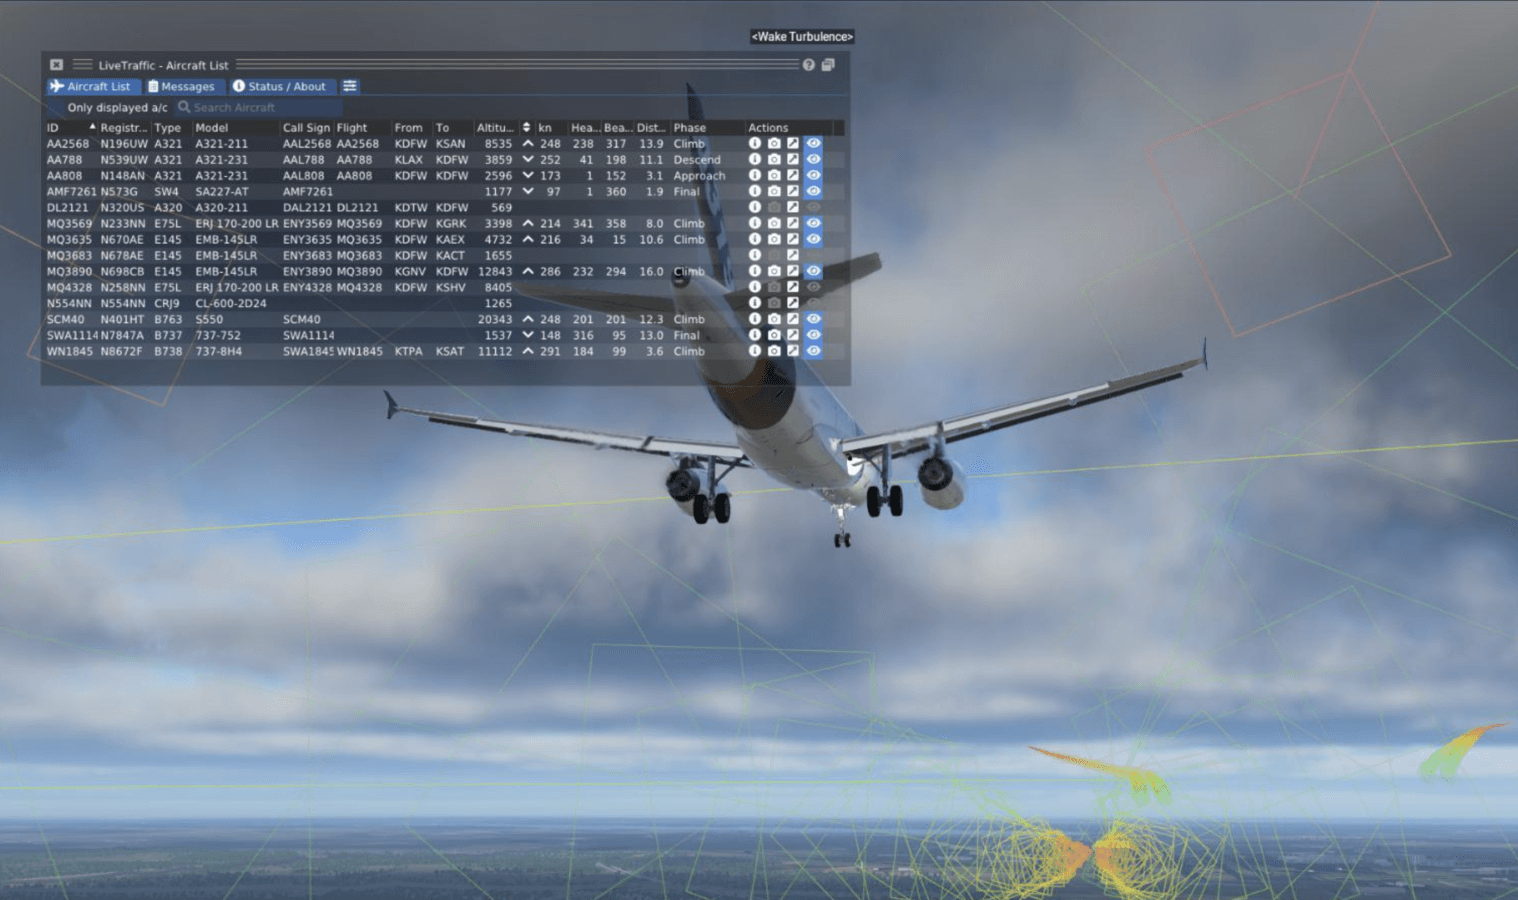
\includegraphics[height=0.5\textheight]{x-plane10-data.png}
	\end{figure}
	\end{columns}
\end{frame}

\begin{frame}{Microcontrollers}
	\begin{figure}
		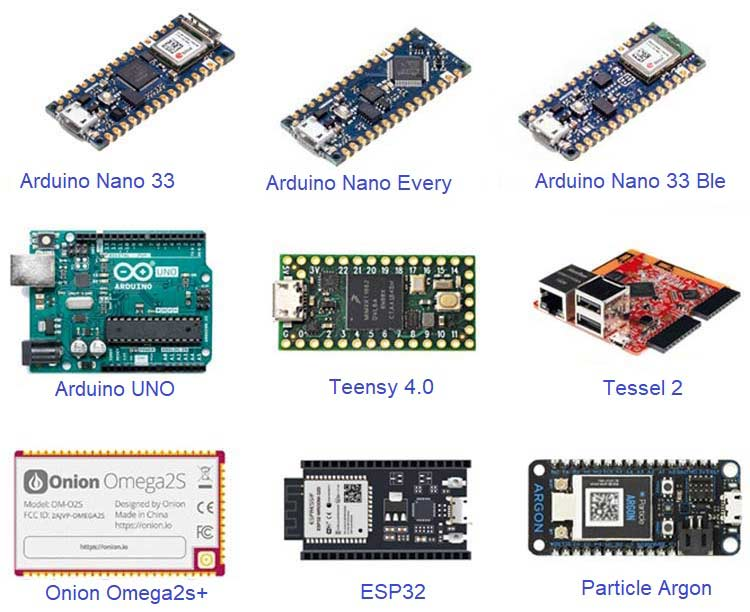
\includegraphics[height=0.7\textheight]{boards.jpg}
	\end{figure}
\end{frame}

\begin{frame}{What for}
\pause
Programmatically control and monitor any aspect of the simulation in real time
\pause
\newline
\newline
Examples
\begin{itemize}
	\item Implement control systems
	\item Develop portable software
\end{itemize}

\end{frame}

\begin{frame}{Main objective}
Establish a communications protocol between X-Plane and microcontrollers
\end{frame}

\begin{frame}{Design decisions}
Based on the context of the simulator at the laboratory and my opinion, the protocol and accompanying software should be
\begin{itemize}
	\item <2-> Easy to use for non-programmers
	\item <3-> Compatible with most simulation software and microcontrollers
	\item <4-> Simple yet powerful 
\end{itemize}
\end{frame}

\begin{frame}{Current solutions}
\pause
\begin{itemize}
	\item NASA’s X-Plane Communications Toolbox
	\item X-Plane built in UDP messaging
	\item Peter Dowson’s Flight Simulator Universal Inter-Process Communication (FSUIPC)
\end{itemize}
\end{frame}

\begin{frame}{1. X-Plane Communications Toolbox}
	\begin{figure}
		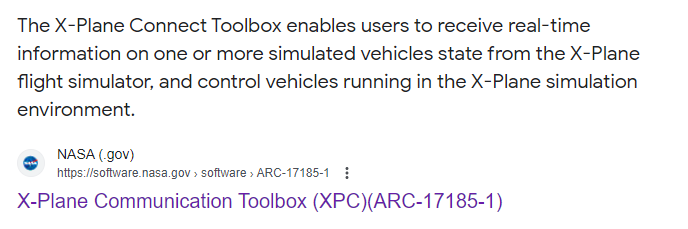
\includegraphics[height=0.5\textheight]{xpc.PNG}
	\end{figure}
\end{frame}

\begin{frame}{1. X-Plane Communications Toolbox}
	Comparison	
	\begin{itemize}
		\item <2-> Has bindings for popular languages
		\item <3-> Works with X-Plane 9, 10 and 11
		\item <4-> Not designed for microcontrollers
		\item <5-> Allows full access to X-Plane data i/o
		\item <6-> Abandoned and buggy
	\end{itemize}
\end{frame}

\begin{frame}{2. X-Plane's built in UDP messaging}
	\begin{figure}
		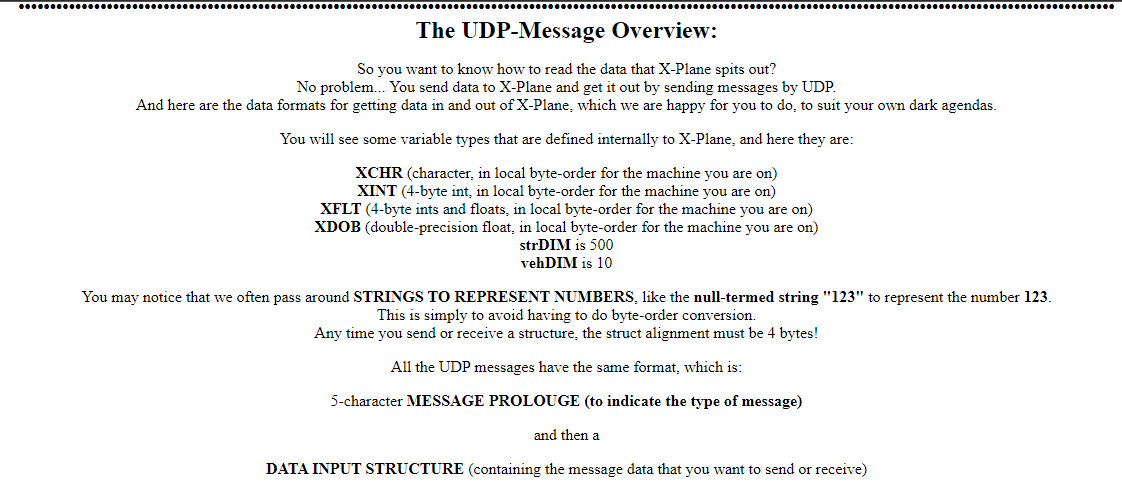
\includegraphics[height=0.8\textheight]{xplaneudp.PNG}
	\end{figure}
\end{frame}

\begin{frame}{2. X-Plane's built in UDP messaging}
	Comparison
	\begin{itemize}
		\item <2-> Difficult to use
		\item <3-> Works with any X-Plane
		\item <4-> Not designed for microcontrollers
		\item <5-> Allows full access to X-Plane data i/o
		\item <6-> Official feature of the simulator
	\end{itemize}
\end{frame}

\begin{frame}{3. FSUIPC}
	Comparison
	\begin{itemize}
		\item <2-> Lots of libraries available yet inconsistent
		\item <3-> Works with on any simulator
		\item <4-> Not designed for microcontrollers
		\item <5-> Allows access to most simulator variables
		\item <6-> Under active development with customer support
	\end{itemize}
\end{frame}

\end{document}